\section{Approach}
\label{sec:approach}

\subsection{Environment and System Architecture}
\label{sub:architecture}

Figure~\ref{fig:architecture} illustrates the environment, placement of Zeroties, and the communication between components.
We describe the parts in the figure refering to the underscored numbers as follows.

\begin{figure}[h]
    \centering
    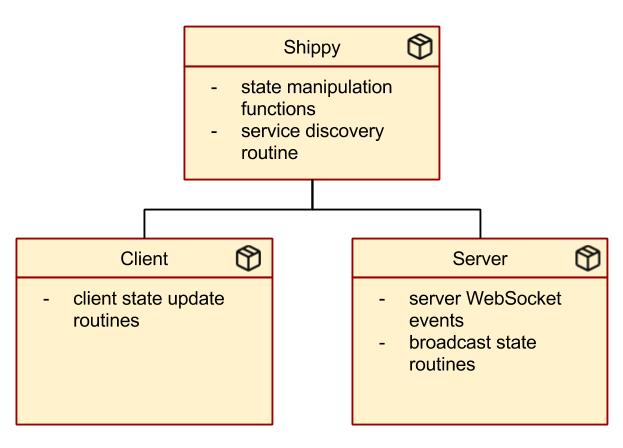
\includegraphics[keepaspectratio,width=6cm]{architecture}
    \caption{System architecture and environment in Zeroties.}
    \label{fig:architecture}
\end{figure}

\begin{enumerate}
\item \textbf{Router}: we use the protocols provided by Zeroconf (\ref{cheshire_2013_dnssd, cheshire_2013_mdns}) for Zeroties. 
In essence, this means that an authoritative list of currently available Zeroties services (as a subset of all Zeroconf services) can be obtained from the router at any given time.

\item \textbf{Hosts}: there can be an arbitrary number of hosts in our local network. A host can be any device in the network with an instance of Zeroties running (i.e. any device with an OS capable of Zeroconf/DNS-SD protocols).

\item \textbf{Zeroties App}: the instance of Zeroties running on this device. 
This is an OS-level application maintaining a list of services.
This list is a mirror of the service list obtained from the router by means of the Zeroconf protocols. 
The list of services constitutes the state of the distributed system~\footnote{Note that there is a clear line between Successorships and Zeroties: Zeroties does not know about the arbitrarily complex state of Successorships or any other app that builds on Zeroties.}

\item \textbf{Browser Addons}: we require browser addons that mediate between web applications and the Zeroties app. These addons expose a JavaScript API to apps built on top of Zeroties.
We have implemented addons for Google Chrome and Mozilla Firefox that constitute such a mediator and we have run Successorships apps with these addons (see Section~\ref{sec:evaluation}).
These addons use Zeroties as a publish/subscribe service.
Note that the Zeroties application itself is not restricted to these addons.
They are only required for web applications running in browsers.
Different applications can use the Zeroties service without these components.

\item \textbf{Publish/Subscribe operations}: applications built on top of Zeroties interact with Zeroties using the common publish/subscribe operations.
\textit{Publish} is the publishing of a Zeroties service and \textit{subscribe} makes the application receive changes to the list of available Zeroties services. 

\item \textbf{Advertisements and service discovery}: the Zeroties application maintains a list of Zeroties services that is obtained from the router.
In a sense, Zeroties acts as a middleware between the router and applications built on top of Zeroties (applications using Successorships as framework being one example). 
Whenever a Zeroties application publishes a service using the Zeroties publish/subscribe API, this will result in the publishing of a service in the network (service advertisement). 
The second part of this communication channel is service discovery.
We describe both service advertisement and service discovery in more detail in Section~\ref{sub:design_goals}
\end{enumerate}


\subsection{Design Decisions}
\label{sub:design}

Zeroties is on system models as in the example described in Section~\ref{sec:background_and_motivation}: local ad-hoc network applications. We claim that there is a dedicated set of such applications, in addition to the document collaboration example, e.g.
\begin{itemize}
\item A project presentation at a meetup where the audience can connect to the presentation and interact with it.
\item An application for printer control in an office
\item An application for the heating system of a hotel
\item Multiplayer mode for browser-based games
\end{itemize}

Such applications have in common a limited number of nodes (generally < 100) and comparably lax requirements for time-to-recovery from system failures: certain downtimes can tolerated as soon as a consistent state is reached eventually.
For example, a running application converging to a consistent state within a time frame of multiple seconds after failures is acceptable.
Our particular goals behind Zeroties are described in the following paragraphs.

\textbf{Replication}. 

In the face of published and removed (or failed) services we want the system to converge to a consistent list of services within 10 seconds.

\subsection{Zeroties API}
\label{sub:zeroties_api}